\documentclass{standalone}
\usepackage{tikz}
\usetikzlibrary{patterns, positioning}
\usepackage[sfdefault]{ClearSans} %% option 'sfdefault' activates Clear Sans as the default text font
\usepackage[T1]{fontenc}

\begin{document}
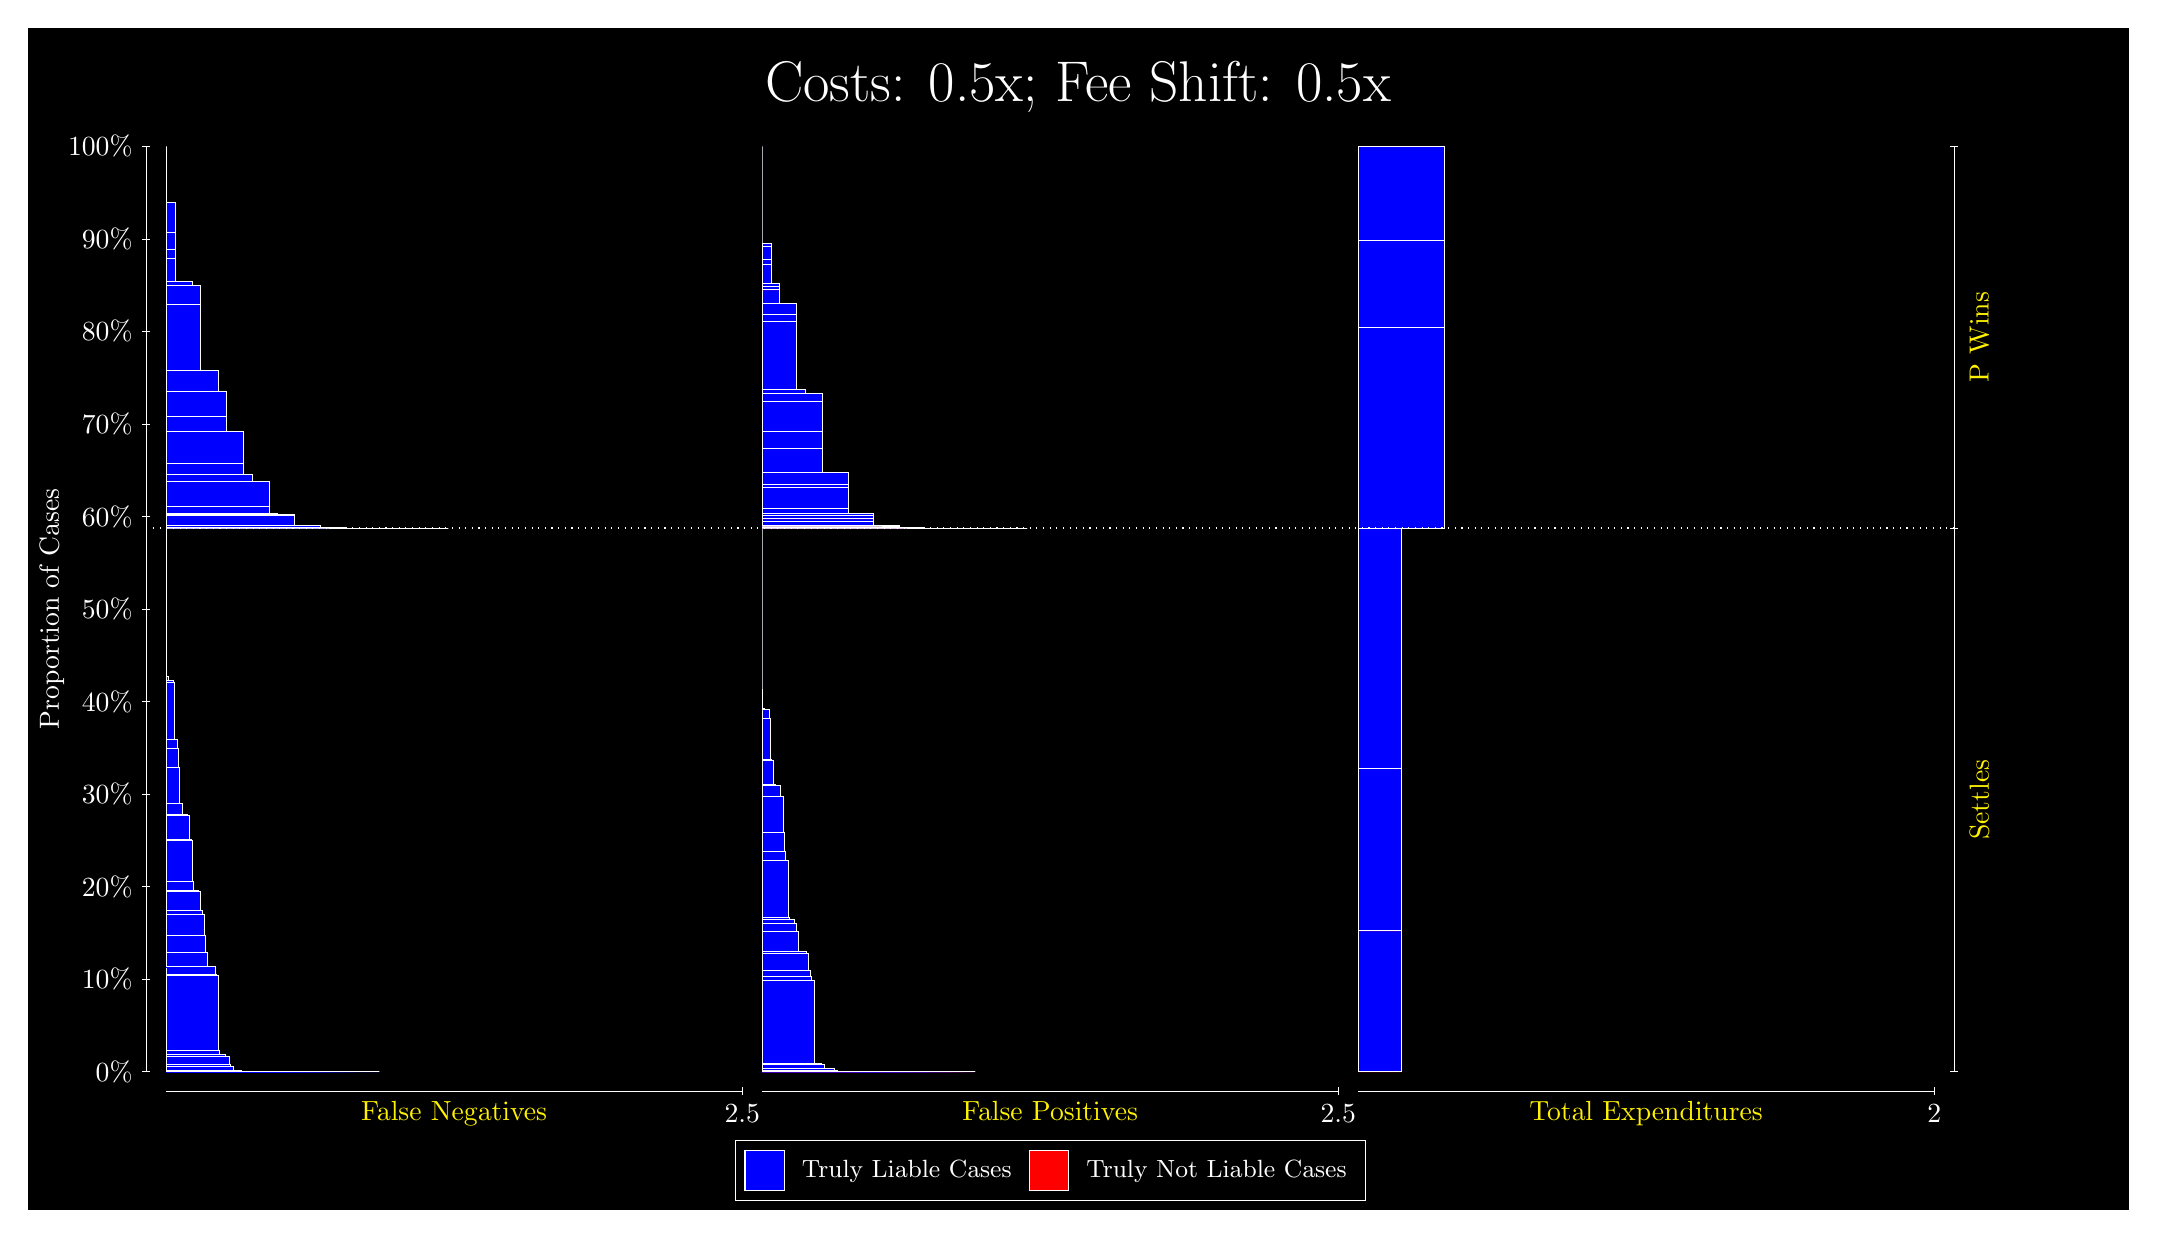
\begin{tikzpicture}
\draw[fill=black] (0,0) rectangle (26.667,15);
\draw[text=white] (0,13.5) rectangle (26.667,15) node[midway] {\huge Costs: 0.5x; Fee Shift: 0.5x};
\draw[white, very thin] (1.5,1.75) -- (1.5,13.5);
\node[rotate=90, text=white, anchor=center] at (0.3, 7.625) {Proportion of Cases};
\draw[white, very thin] (1.45,1.75) -- (1.55,1.75);
\node[text=white, anchor=east] at (1.45, 1.75) {0\%};
\draw[white, very thin] (1.45,2.925) -- (1.55,2.925);
\node[text=white, anchor=east] at (1.45, 2.925) {10\%};
\draw[white, very thin] (1.45,4.1) -- (1.55,4.1);
\node[text=white, anchor=east] at (1.45, 4.1) {20\%};
\draw[white, very thin] (1.45,5.275) -- (1.55,5.275);
\node[text=white, anchor=east] at (1.45, 5.275) {30\%};
\draw[white, very thin] (1.45,6.45) -- (1.55,6.45);
\node[text=white, anchor=east] at (1.45, 6.45) {40\%};
\draw[white, very thin] (1.45,7.625) -- (1.55,7.625);
\node[text=white, anchor=east] at (1.45, 7.625) {50\%};
\draw[white, very thin] (1.45,8.8) -- (1.55,8.8);
\node[text=white, anchor=east] at (1.45, 8.8) {60\%};
\draw[white, very thin] (1.45,9.975) -- (1.55,9.975);
\node[text=white, anchor=east] at (1.45, 9.975) {70\%};
\draw[white, very thin] (1.45,11.15) -- (1.55,11.15);
\node[text=white, anchor=east] at (1.45, 11.15) {80\%};
\draw[white, very thin] (1.45,12.325) -- (1.55,12.325);
\node[text=white, anchor=east] at (1.45, 12.325) {90\%};
\draw[white, very thin] (1.45,13.5) -- (1.55,13.5);
\node[text=white, anchor=east] at (1.45, 13.5) {100\%};

\draw[white, very thin] (24.457,1.75) -- (24.457,13.5);
\draw[white, very thin] (24.407,1.75) -- (24.507,1.75);
\node[anchor=west] at (24.407, 1.75) {};
\draw[white, very thin] (24.407,8.6529) -- (24.507,8.6529);
\node[anchor=west] at (24.407, 8.6529) {};
\draw[white, very thin] (24.407,13.5) -- (24.507,13.5);
\node[anchor=west] at (24.407, 13.5) {};

\draw[white, very thin, fill=blue] (1.75,1.75) rectangle (4.458,1.75);
\draw[white, very thin, fill=blue] (1.75,1.75) rectangle (4.1652,1.75);
\draw[white, very thin, fill=blue] (1.75,1.75) rectangle (4.1327,1.75);
\draw[white, very thin, fill=blue] (1.75,1.75) rectangle (4.0188,1.75);
\draw[white, very thin, fill=blue] (1.75,1.75) rectangle (3.8725,1.75);
\draw[white, very thin, fill=blue] (1.75,1.75) rectangle (3.8399,1.75);
\draw[white, very thin, fill=blue] (1.75,1.75) rectangle (3.8074,1.75);
\draw[white, very thin, fill=blue] (1.75,1.75) rectangle (3.7261,1.75);
\draw[white, very thin, fill=blue] (1.75,1.75) rectangle (3.6936,1.75);
\draw[white, very thin, fill=blue] (1.75,1.75) rectangle (3.5797,1.75);
\draw[white, very thin, fill=blue] (1.75,1.75) rectangle (3.5472,1.75);
\draw[white, very thin, fill=blue] (1.75,1.75) rectangle (3.5147,1.75);
\draw[white, very thin, fill=blue] (1.75,1.75) rectangle (3.4821,1.75);
\draw[white, very thin, fill=blue] (1.75,1.75) rectangle (3.4333,1.75);
\draw[white, very thin, fill=blue] (1.75,1.75) rectangle (3.4008,1.75);
\draw[white, very thin, fill=blue] (1.75,1.75) rectangle (3.3683,1.75);
\draw[white, very thin, fill=blue] (1.75,1.75) rectangle (3.287,1.75);
\draw[white, very thin, fill=blue] (1.75,1.75) rectangle (3.2544,1.75);
\draw[white, very thin, fill=blue] (1.75,1.75) rectangle (3.2219,1.75);
\draw[white, very thin, fill=blue] (1.75,1.75) rectangle (3.1894,1.75);
\draw[white, very thin, fill=blue] (1.75,1.75) rectangle (3.1568,1.75);
\draw[white, very thin, fill=blue] (1.75,1.75) rectangle (3.1406,1.75);
\draw[white, very thin, fill=blue] (1.75,1.75) rectangle (3.1081,1.75);
\draw[white, very thin, fill=blue] (1.75,1.75) rectangle (3.0755,1.7501);
\draw[white, very thin, fill=blue] (1.75,1.7501) rectangle (3.043,1.7501);
\draw[white, very thin, fill=blue] (1.75,1.7501) rectangle (2.9942,1.7501);
\draw[white, very thin, fill=blue] (1.75,1.7501) rectangle (2.9617,1.7501);
\draw[white, very thin, fill=blue] (1.75,1.7501) rectangle (2.9292,1.7523);
\draw[white, very thin, fill=blue] (1.75,1.7523) rectangle (2.8966,1.7528);
\draw[white, very thin, fill=blue] (1.75,1.7528) rectangle (2.8641,1.7528);
\draw[white, very thin, fill=blue] (1.75,1.7528) rectangle (2.8316,1.7533);
\draw[white, very thin, fill=blue] (1.75,1.7533) rectangle (2.8153,1.7534);
\draw[white, very thin, fill=blue] (1.75,1.7534) rectangle (2.7828,1.7534);
\draw[white, very thin, fill=blue] (1.75,1.7534) rectangle (2.7502,1.758);
\draw[white, very thin, fill=blue] (1.75,1.758) rectangle (2.7177,1.7581);
\draw[white, very thin, fill=blue] (1.75,1.7581) rectangle (2.7015,1.7681);
\draw[white, very thin, fill=blue] (1.75,1.7681) rectangle (2.6689,1.7683);
\draw[white, very thin, fill=blue] (1.75,1.7683) rectangle (2.6364,1.7684);
\draw[white, very thin, fill=blue] (1.75,1.7684) rectangle (2.6039,1.8129);
\draw[white, very thin, fill=blue] (1.75,1.8129) rectangle (2.5713,1.8365);
\draw[white, very thin, fill=blue] (1.75,1.8365) rectangle (2.5551,1.9391);
\draw[white, very thin, fill=blue] (1.75,1.9391) rectangle (2.5388,1.9436);
\draw[white, very thin, fill=blue] (1.75,1.9436) rectangle (2.5063,1.9678);
\draw[white, very thin, fill=blue] (1.75,1.9678) rectangle (2.49,1.9706);
\draw[white, very thin, fill=blue] (1.75,1.9706) rectangle (2.4575,1.9706);
\draw[white, very thin, fill=blue] (1.75,1.9706) rectangle (2.425,2.0194);
\draw[white, very thin, fill=blue] (1.75,2.0194) rectangle (2.4087,2.9784);
\draw[white, very thin, fill=blue] (1.75,2.9784) rectangle (2.3924,2.9806);
\draw[white, very thin, fill=blue] (1.75,2.9806) rectangle (2.3762,3.0811);
\draw[white, very thin, fill=blue] (1.75,3.0811) rectangle (2.3436,3.0833);
\draw[white, very thin, fill=blue] (1.75,3.0833) rectangle (2.3111,3.085);
\draw[white, very thin, fill=blue] (1.75,3.085) rectangle (2.2786,3.2625);
\draw[white, very thin, fill=blue] (1.75,3.2625) rectangle (2.2461,3.4844);
\draw[white, very thin, fill=blue] (1.75,3.4844) rectangle (2.2298,3.7442);
\draw[white, very thin, fill=blue] (1.75,3.7442) rectangle (2.2135,3.7931);
\draw[white, very thin, fill=blue] (1.75,3.7931) rectangle (2.181,4.0396);
\draw[white, very thin, fill=blue] (1.75,4.0396) rectangle (2.1647,4.0573);
\draw[white, very thin, fill=blue] (1.75,4.0573) rectangle (2.1322,4.0573);
\draw[white, very thin, fill=blue] (1.75,4.0573) rectangle (2.0997,4.1647);
\draw[white, very thin, fill=blue] (1.75,4.1647) rectangle (2.0834,4.6912);
\draw[white, very thin, fill=blue] (1.75,4.6912) rectangle (2.0672,4.6964);
\draw[white, very thin, fill=blue] (1.75,4.6964) rectangle (2.0509,5.0086);
\draw[white, very thin, fill=blue] (1.75,5.0086) rectangle (2.0184,5.0133);
\draw[white, very thin, fill=blue] (1.75,5.0133) rectangle (1.9858,5.0181);
\draw[white, very thin, fill=blue] (1.75,5.0181) rectangle (1.9533,5.1541);
\draw[white, very thin, fill=blue] (1.75,5.1541) rectangle (1.9208,5.6128);
\draw[white, very thin, fill=blue] (1.75,5.6128) rectangle (1.9045,5.8593);
\draw[white, very thin, fill=blue] (1.75,5.8593) rectangle (1.8882,5.9681);
\draw[white, very thin, fill=blue] (1.75,5.9681) rectangle (1.8557,6.6983);
\draw[white, very thin, fill=blue] (1.75,6.6983) rectangle (1.8395,6.716);
\draw[white, very thin, fill=blue] (1.75,6.716) rectangle (1.8069,6.716);
\draw[white, very thin, fill=blue] (1.75,6.716) rectangle (1.7744,6.7649);
\draw[white, very thin, fill=blue] (1.75,6.7649) rectangle (1.7581,6.8736);
\draw[white, very thin, fill=red] (1.75,6.8736) rectangle (1.75,6.8736);
\draw[white, very thin, fill=blue] (1.75,6.8736) rectangle (1.75,8.6529);
\draw[white, very thin, fill=blue] (1.75,8.6529) rectangle (5.3362,8.6529);
\draw[white, very thin, fill=blue] (1.75,8.6529) rectangle (5.011,8.6529);
\draw[white, very thin, fill=blue] (1.75,8.6529) rectangle (4.6857,8.6529);
\draw[white, very thin, fill=blue] (1.75,8.6529) rectangle (4.4661,8.6529);
\draw[white, very thin, fill=blue] (1.75,8.6529) rectangle (4.3604,8.6531);
\draw[white, very thin, fill=blue] (1.75,8.6531) rectangle (4.1408,8.6531);
\draw[white, very thin, fill=blue] (1.75,8.6531) rectangle (4.0351,8.655);
\draw[white, very thin, fill=blue] (1.75,8.655) rectangle (4.0351,8.6564);
\draw[white, very thin, fill=blue] (1.75,8.6564) rectangle (3.8155,8.6564);
\draw[white, very thin, fill=blue] (1.75,8.6564) rectangle (3.8155,8.6564);
\draw[white, very thin, fill=blue] (1.75,8.6564) rectangle (3.7098,8.668);
\draw[white, very thin, fill=blue] (1.75,8.668) rectangle (3.7098,8.6847);
\draw[white, very thin, fill=blue] (1.75,8.6847) rectangle (3.4903,8.6849);
\draw[white, very thin, fill=blue] (1.75,8.6849) rectangle (3.3845,8.8203);
\draw[white, very thin, fill=blue] (1.75,8.8203) rectangle (3.3845,8.8295);
\draw[white, very thin, fill=blue] (1.75,8.8295) rectangle (3.165,8.8307);
\draw[white, very thin, fill=blue] (1.75,8.8307) rectangle (3.165,8.8345);
\draw[white, very thin, fill=blue] (1.75,8.8345) rectangle (3.0593,8.9277);
\draw[white, very thin, fill=blue] (1.75,8.9277) rectangle (3.0593,9.2502);
\draw[white, very thin, fill=blue] (1.75,9.2502) rectangle (2.8397,9.3399);
\draw[white, very thin, fill=blue] (1.75,9.3399) rectangle (2.734,9.4777);
\draw[white, very thin, fill=blue] (1.75,9.4777) rectangle (2.734,9.8779);
\draw[white, very thin, fill=blue] (1.75,9.8779) rectangle (2.734,9.8819);
\draw[white, very thin, fill=blue] (1.75,9.8819) rectangle (2.5144,10.068);
\draw[white, very thin, fill=blue] (1.75,10.068) rectangle (2.5144,10.391);
\draw[white, very thin, fill=blue] (1.75,10.391) rectangle (2.4087,10.652);
\draw[white, very thin, fill=blue] (1.75,10.652) rectangle (2.1891,11.497);
\draw[white, very thin, fill=blue] (1.75,11.497) rectangle (2.1891,11.74);
\draw[white, very thin, fill=blue] (1.75,11.74) rectangle (2.0834,11.74);
\draw[white, very thin, fill=blue] (1.75,11.74) rectangle (2.0834,11.785);
\draw[white, very thin, fill=blue] (1.75,11.785) rectangle (2.0834,11.785);
\draw[white, very thin, fill=blue] (1.75,11.785) rectangle (1.8638,12.074);
\draw[white, very thin, fill=blue] (1.75,12.074) rectangle (1.8638,12.194);
\draw[white, very thin, fill=blue] (1.75,12.194) rectangle (1.8638,12.409);
\draw[white, very thin, fill=blue] (1.75,12.409) rectangle (1.8638,12.795);
\draw[white, very thin, fill=blue] (1.75,12.795) rectangle (1.7581,12.795);
\draw[white, very thin, fill=blue] (1.75,12.795) rectangle (1.7581,12.795);
\draw[white, very thin, fill=red] (1.75,12.795) rectangle (1.75,12.795);
\draw[white, very thin, fill=blue] (1.75,12.795) rectangle (1.75,13.5);
\draw[white, very thin, fill=red] (9.3189,1.75) rectangle (12.027,1.75);
\draw[white, very thin, fill=blue] (9.3189,1.75) rectangle (12.027,1.75);
\draw[white, very thin, fill=red] (9.3189,1.75) rectangle (11.88,1.75);
\draw[white, very thin, fill=blue] (9.3189,1.75) rectangle (11.88,1.75);
\draw[white, very thin, fill=red] (9.3189,1.75) rectangle (11.734,1.75);
\draw[white, very thin, fill=blue] (9.3189,1.75) rectangle (11.734,1.75);
\draw[white, very thin, fill=blue] (9.3189,1.75) rectangle (11.702,1.75);
\draw[white, very thin, fill=blue] (9.3189,1.75) rectangle (11.555,1.75);
\draw[white, very thin, fill=red] (9.3189,1.75) rectangle (11.441,1.75);
\draw[white, very thin, fill=blue] (9.3189,1.75) rectangle (11.441,1.75);
\draw[white, very thin, fill=blue] (9.3189,1.75) rectangle (11.409,1.75);
\draw[white, very thin, fill=blue] (9.3189,1.75) rectangle (11.376,1.75);
\draw[white, very thin, fill=red] (9.3189,1.75) rectangle (11.295,1.75);
\draw[white, very thin, fill=blue] (9.3189,1.75) rectangle (11.295,1.75);
\draw[white, very thin, fill=blue] (9.3189,1.75) rectangle (11.23,1.75);
\draw[white, very thin, fill=red] (9.3189,1.75) rectangle (11.149,1.75);
\draw[white, very thin, fill=blue] (9.3189,1.75) rectangle (11.149,1.75);
\draw[white, very thin, fill=blue] (9.3189,1.75) rectangle (11.116,1.75);
\draw[white, very thin, fill=blue] (9.3189,1.75) rectangle (11.084,1.75);
\draw[white, very thin, fill=blue] (9.3189,1.75) rectangle (11.051,1.75);
\draw[white, very thin, fill=red] (9.3189,1.75) rectangle (11.002,1.75);
\draw[white, very thin, fill=blue] (9.3189,1.75) rectangle (11.002,1.75);
\draw[white, very thin, fill=blue] (9.3189,1.75) rectangle (10.97,1.75);
\draw[white, very thin, fill=blue] (9.3189,1.75) rectangle (10.905,1.75);
\draw[white, very thin, fill=red] (9.3189,1.75) rectangle (10.856,1.75);
\draw[white, very thin, fill=blue] (9.3189,1.75) rectangle (10.856,1.75);
\draw[white, very thin, fill=blue] (9.3189,1.75) rectangle (10.823,1.75);
\draw[white, very thin, fill=blue] (9.3189,1.75) rectangle (10.791,1.75);
\draw[white, very thin, fill=blue] (9.3189,1.75) rectangle (10.758,1.75);
\draw[white, very thin, fill=blue] (9.3189,1.75) rectangle (10.726,1.75);
\draw[white, very thin, fill=red] (9.3189,1.75) rectangle (10.709,1.75);
\draw[white, very thin, fill=blue] (9.3189,1.75) rectangle (10.709,1.75);
\draw[white, very thin, fill=blue] (9.3189,1.75) rectangle (10.677,1.75);
\draw[white, very thin, fill=blue] (9.3189,1.75) rectangle (10.644,1.75);
\draw[white, very thin, fill=blue] (9.3189,1.75) rectangle (10.579,1.7501);
\draw[white, very thin, fill=red] (9.3189,1.7501) rectangle (10.563,1.7501);
\draw[white, very thin, fill=blue] (9.3189,1.7501) rectangle (10.563,1.7511);
\draw[white, very thin, fill=blue] (9.3189,1.7511) rectangle (10.531,1.7511);
\draw[white, very thin, fill=blue] (9.3189,1.7511) rectangle (10.498,1.7511);
\draw[white, very thin, fill=blue] (9.3189,1.7511) rectangle (10.465,1.7511);
\draw[white, very thin, fill=blue] (9.3189,1.7511) rectangle (10.433,1.7533);
\draw[white, very thin, fill=red] (9.3189,1.7533) rectangle (10.417,1.7533);
\draw[white, very thin, fill=blue] (9.3189,1.7533) rectangle (10.417,1.7533);
\draw[white, very thin, fill=blue] (9.3189,1.7533) rectangle (10.4,1.7533);
\draw[white, very thin, fill=blue] (9.3189,1.7533) rectangle (10.384,1.7534);
\draw[white, very thin, fill=blue] (9.3189,1.7534) rectangle (10.352,1.7534);
\draw[white, very thin, fill=blue] (9.3189,1.7534) rectangle (10.319,1.7535);
\draw[white, very thin, fill=red] (9.3189,1.7535) rectangle (10.27,1.7535);
\draw[white, very thin, fill=blue] (9.3189,1.7535) rectangle (10.27,1.763);
\draw[white, very thin, fill=blue] (9.3189,1.763) rectangle (10.254,1.768);
\draw[white, very thin, fill=blue] (9.3189,1.768) rectangle (10.238,1.7952);
\draw[white, very thin, fill=blue] (9.3189,1.7952) rectangle (10.205,1.7956);
\draw[white, very thin, fill=blue] (9.3189,1.7956) rectangle (10.173,1.7958);
\draw[white, very thin, fill=blue] (9.3189,1.7958) rectangle (10.14,1.7959);
\draw[white, very thin, fill=blue] (9.3189,1.7959) rectangle (10.108,1.8447);
\draw[white, very thin, fill=blue] (9.3189,1.8447) rectangle (10.091,1.8449);
\draw[white, very thin, fill=blue] (9.3189,1.8449) rectangle (10.075,1.8501);
\draw[white, very thin, fill=blue] (9.3189,1.8501) rectangle (10.059,1.8547);
\draw[white, very thin, fill=blue] (9.3189,1.8547) rectangle (10.026,1.8547);
\draw[white, very thin, fill=blue] (9.3189,1.8547) rectangle (9.9938,1.8575);
\draw[white, very thin, fill=red] (9.3189,1.8575) rectangle (9.9776,1.8575);
\draw[white, very thin, fill=blue] (9.3189,1.8575) rectangle (9.9776,2.9094);
\draw[white, very thin, fill=blue] (9.3189,2.9094) rectangle (9.945,2.9655);
\draw[white, very thin, fill=blue] (9.3189,2.9655) rectangle (9.9288,3.0333);
\draw[white, very thin, fill=blue] (9.3189,3.0333) rectangle (9.9125,3.258);
\draw[white, very thin, fill=blue] (9.3189,3.258) rectangle (9.88,3.277);
\draw[white, very thin, fill=blue] (9.3189,3.277) rectangle (9.8475,3.2791);
\draw[white, very thin, fill=blue] (9.3189,3.2791) rectangle (9.8149,3.2808);
\draw[white, very thin, fill=blue] (9.3189,3.2808) rectangle (9.7824,3.527);
\draw[white, very thin, fill=blue] (9.3189,3.527) rectangle (9.7661,3.5293);
\draw[white, very thin, fill=blue] (9.3189,3.5293) rectangle (9.7499,3.638);
\draw[white, very thin, fill=blue] (9.3189,3.638) rectangle (9.7336,3.6869);
\draw[white, very thin, fill=blue] (9.3189,3.6869) rectangle (9.7011,3.6869);
\draw[white, very thin, fill=blue] (9.3189,3.6869) rectangle (9.6685,3.7046);
\draw[white, very thin, fill=blue] (9.3189,3.7046) rectangle (9.6523,4.4348);
\draw[white, very thin, fill=blue] (9.3189,4.4348) rectangle (9.6198,4.5436);
\draw[white, very thin, fill=blue] (9.3189,4.5436) rectangle (9.6035,4.79);
\draw[white, very thin, fill=blue] (9.3189,4.79) rectangle (9.5872,5.2487);
\draw[white, very thin, fill=blue] (9.3189,5.2487) rectangle (9.5547,5.3848);
\draw[white, very thin, fill=blue] (9.3189,5.3848) rectangle (9.5222,5.3895);
\draw[white, very thin, fill=blue] (9.3189,5.3895) rectangle (9.4896,5.3943);
\draw[white, very thin, fill=blue] (9.3189,5.3943) rectangle (9.4571,5.7065);
\draw[white, very thin, fill=blue] (9.3189,5.7065) rectangle (9.4408,5.7117);
\draw[white, very thin, fill=blue] (9.3189,5.7117) rectangle (9.4246,6.2382);
\draw[white, very thin, fill=blue] (9.3189,6.2382) rectangle (9.4083,6.3456);
\draw[white, very thin, fill=blue] (9.3189,6.3456) rectangle (9.3758,6.3456);
\draw[white, very thin, fill=blue] (9.3189,6.3456) rectangle (9.3433,6.3633);
\draw[white, very thin, fill=blue] (9.3189,6.3633) rectangle (9.327,6.6098);
\draw[white, very thin, fill=blue] (9.3189,6.6098) rectangle (9.3189,8.6529);
\draw[white, very thin, fill=red] (9.3189,8.6529) rectangle (12.686,8.6529);
\draw[white, very thin, fill=blue] (9.3189,8.6529) rectangle (12.686,8.6529);
\draw[white, very thin, fill=red] (9.3189,8.6529) rectangle (12.36,8.6529);
\draw[white, very thin, fill=blue] (9.3189,8.6529) rectangle (12.36,8.6529);
\draw[white, very thin, fill=red] (9.3189,8.6529) rectangle (12.035,8.6529);
\draw[white, very thin, fill=blue] (9.3189,8.6529) rectangle (12.035,8.6529);
\draw[white, very thin, fill=blue] (9.3189,8.6529) rectangle (12.035,8.6529);
\draw[white, very thin, fill=blue] (9.3189,8.6529) rectangle (12.035,8.6529);
\draw[white, very thin, fill=red] (9.3189,8.6529) rectangle (11.71,8.6529);
\draw[white, very thin, fill=blue] (9.3189,8.6529) rectangle (11.71,8.653);
\draw[white, very thin, fill=blue] (9.3189,8.653) rectangle (11.71,8.6531);
\draw[white, very thin, fill=red] (9.3189,8.6531) rectangle (11.49,8.6531);
\draw[white, very thin, fill=blue] (9.3189,8.6531) rectangle (11.49,8.6531);
\draw[white, very thin, fill=red] (9.3189,8.6531) rectangle (11.384,8.6531);
\draw[white, very thin, fill=blue] (9.3189,8.6531) rectangle (11.384,8.6541);
\draw[white, very thin, fill=blue] (9.3189,8.6541) rectangle (11.384,8.6562);
\draw[white, very thin, fill=red] (9.3189,8.6562) rectangle (11.165,8.6562);
\draw[white, very thin, fill=blue] (9.3189,8.6562) rectangle (11.165,8.6562);
\draw[white, very thin, fill=blue] (9.3189,8.6562) rectangle (11.059,8.6647);
\draw[white, very thin, fill=red] (9.3189,8.6647) rectangle (11.059,8.6647);
\draw[white, very thin, fill=blue] (9.3189,8.6647) rectangle (11.059,8.6714);
\draw[white, very thin, fill=blue] (9.3189,8.6714) rectangle (11.059,8.6845);
\draw[white, very thin, fill=red] (9.3189,8.6845) rectangle (10.84,8.6845);
\draw[white, very thin, fill=blue] (9.3189,8.6845) rectangle (10.84,8.6845);
\draw[white, very thin, fill=blue] (9.3189,8.6845) rectangle (10.734,8.7344);
\draw[white, very thin, fill=blue] (9.3189,8.7344) rectangle (10.734,8.7725);
\draw[white, very thin, fill=red] (9.3189,8.7725) rectangle (10.734,8.7725);
\draw[white, very thin, fill=blue] (9.3189,8.7725) rectangle (10.734,8.8093);
\draw[white, very thin, fill=blue] (9.3189,8.8093) rectangle (10.734,8.8415);
\draw[white, very thin, fill=red] (9.3189,8.8415) rectangle (10.514,8.8415);
\draw[white, very thin, fill=blue] (9.3189,8.8415) rectangle (10.514,8.8415);
\draw[white, very thin, fill=blue] (9.3189,8.8415) rectangle (10.514,8.8415);
\draw[white, very thin, fill=blue] (9.3189,8.8415) rectangle (10.409,8.9053);
\draw[white, very thin, fill=red] (9.3189,8.9053) rectangle (10.409,8.9053);
\draw[white, very thin, fill=blue] (9.3189,8.9053) rectangle (10.409,9.1647);
\draw[white, very thin, fill=blue] (9.3189,9.1647) rectangle (10.409,9.2122);
\draw[white, very thin, fill=blue] (9.3189,9.2122) rectangle (10.409,9.358);
\draw[white, very thin, fill=red] (9.3189,9.358) rectangle (10.189,9.358);
\draw[white, very thin, fill=blue] (9.3189,9.358) rectangle (10.189,9.3581);
\draw[white, very thin, fill=blue] (9.3189,9.3581) rectangle (10.189,9.3581);
\draw[white, very thin, fill=blue] (9.3189,9.3581) rectangle (10.083,9.6713);
\draw[white, very thin, fill=blue] (9.3189,9.6713) rectangle (10.083,9.8819);
\draw[white, very thin, fill=blue] (9.3189,9.8819) rectangle (10.083,10.257);
\draw[white, very thin, fill=blue] (9.3189,10.257) rectangle (10.083,10.368);
\draw[white, very thin, fill=red] (9.3189,10.368) rectangle (9.8637,10.368);
\draw[white, very thin, fill=blue] (9.3189,10.368) rectangle (9.8637,10.411);
\draw[white, very thin, fill=blue] (9.3189,10.411) rectangle (9.8637,10.412);
\draw[white, very thin, fill=blue] (9.3189,10.412) rectangle (9.8637,10.413);
\draw[white, very thin, fill=blue] (9.3189,10.413) rectangle (9.758,11.28);
\draw[white, very thin, fill=blue] (9.3189,11.28) rectangle (9.758,11.369);
\draw[white, very thin, fill=blue] (9.3189,11.369) rectangle (9.758,11.501);
\draw[white, very thin, fill=blue] (9.3189,11.501) rectangle (9.5384,11.681);
\draw[white, very thin, fill=red] (9.3189,11.681) rectangle (9.5384,11.681);
\draw[white, very thin, fill=blue] (9.3189,11.681) rectangle (9.5384,11.728);
\draw[white, very thin, fill=blue] (9.3189,11.728) rectangle (9.5384,11.762);
\draw[white, very thin, fill=blue] (9.3189,11.762) rectangle (9.4327,11.996);
\draw[white, very thin, fill=blue] (9.3189,11.996) rectangle (9.4327,12.068);
\draw[white, very thin, fill=blue] (9.3189,12.068) rectangle (9.4327,12.236);
\draw[white, very thin, fill=blue] (9.3189,12.236) rectangle (9.4327,12.271);
\draw[white, very thin, fill=blue] (9.3189,12.271) rectangle (9.3189,13.5);
\draw[white, very thin, fill=red] (16.888,1.75) rectangle (17.437,1.75);
\draw[white, very thin, fill=blue] (16.888,1.75) rectangle (17.437,3.5396);
\draw[white, very thin, fill=red] (16.888,3.5396) rectangle (17.437,3.5396);
\draw[white, very thin, fill=blue] (16.888,3.5396) rectangle (17.437,5.6017);
\draw[white, very thin, fill=red] (16.888,5.6017) rectangle (17.437,5.6017);
\draw[white, very thin, fill=blue] (16.888,5.6017) rectangle (17.437,8.6529);
\draw[white, very thin, fill=red] (16.888,8.6529) rectangle (17.986,8.6529);
\draw[white, very thin, fill=blue] (16.888,8.6529) rectangle (17.986,11.203);
\draw[white, very thin, fill=red] (16.888,11.203) rectangle (17.986,11.203);
\draw[white, very thin, fill=blue] (16.888,11.203) rectangle (17.986,12.305);
\draw[white, very thin, fill=red] (16.888,12.305) rectangle (17.986,12.305);
\draw[white, very thin, fill=blue] (16.888,12.305) rectangle (17.986,13.5);
\draw[white, dotted] (1.5,8.6529) -- (24.457,8.6529);
\draw[white, very thin] (1.75,1.5) -- (9.0689,1.5);
\node[text=yellow, anchor=north] at (5.4094, 1.5) {False Negatives};
\draw[white, very thin] (9.0689,1.45) -- (9.0689,1.55);
\node[text=white, anchor=north] at (9.0689, 1.45) {2.5};

\draw[white, very thin] (9.3189,1.5) -- (16.638,1.5);
\node[text=yellow, anchor=north] at (12.978, 1.5) {False Positives};
\draw[white, very thin] (16.638,1.45) -- (16.638,1.55);
\node[text=white, anchor=north] at (16.638, 1.45) {2.5};

\draw[white, very thin] (16.888,1.5) -- (24.207,1.5);
\node[text=yellow, anchor=north] at (20.547, 1.5) {Total Expenditures};
\draw[white, very thin] (24.207,1.45) -- (24.207,1.55);
\node[text=white, anchor=north] at (24.207, 1.45) {2};

\node[text=yellow, centered, rotate=90] at (24.777, 5.2014) {Settles};
\node[text=yellow, centered, rotate=90] at (24.777, 11.076) {P Wins};

\draw (12.978300999999998,1.5) node[draw=none] (baseCoordinate) {};
\begin{scope}[align=center]
        \matrix[scale=0.5, draw=white, below=0.5cm of baseCoordinate, nodes={draw}, column sep=0.1cm]{
            \node[rectangle, draw, minimum width=0.5cm, minimum height=0.5cm, fill=blue] {}; &
            \node[draw=none, font=\small, text=white] (B) {Truly Liable Cases}; &
            \node[rectangle, draw, minimum width=0.5cm, minimum height=0.5cm, fill=red] {}; &
            \node[draw=none, font=\small, text=white] (B) {Truly Not Liable Cases}; \\
            };
\end{scope}

\end{tikzpicture}
\end{document}